\section{Веса IV c}
\subsection{Условие задания}
В графе могут быть циклы отрицательного веса.

\textbf{Вариант 10:} Вывести кратчайший путь из вершины $u$ до вершины $v$.

\subsection{Примеры исходного кода}
Для выполнения задания был реализован метод\\
\mitext{taskTen()}:
\begin{minted}{typescript}
/**
 * Метод, который находит кратчайший путь между двумя данными
 * вершинами `u` и `v`. В графе могут быть отрицательные циклы.
 * Реализация построена на алгоритме Флойда.
 * @param u начальная вершина
 * @param v конечная вершина
 */
taskTen(u: string, v: string): { distance: number; path: string[] } {
  if (!this.exists(u)) {
    throw new NodeNotExists(u)
  }
  if (!this.exists(v)) {
    throw new NodeNotExists(v)
  }

  // Map, связывающая строковую метку вершины с числом
  const indexOf = new Map(Array.from(this.adj.keys()).map((v, i) => [v, i]))
  const labelOf = new Map(Array.from(this.adj.keys()).map((v, i) => [i, v]))
  // Список смежности, только метки теперь числа
  const adj = new Map(Array.from(this.adj.entries()).map((v, i) =>
    [i, new Map(Array.from(v[1]).map(v => [indexOf.get(v[0])!, v[1]]))]
  ))
  const vertices = Array.from(adj.keys())

  // инициализировать матрицу расстояний и матрицу следующих вершин
  const dist: number[][] = []
  const next: (number | null)[][] = []

  for (const i of vertices) {
    dist[i] = []
    next[i] = []
    for (const j of vertices) {
      dist[i][j] = i === j ? 0 : Infinity
      next[i][j] = null
    }
  }

  // заполнить матрицу расстояний на основе весов списка смежности
  for (const [src, neighbors] of adj.entries()) {
    for (const [dst, weight] of neighbors.entries()) {
      dist[src][dst] = weight
      next[src][dst] = dst // установить следующую вершину в соответствии с ребром
    }
  }

  // алгоритм Флойда
  for (const k of vertices) {
    for (const i of vertices) {
      for (const j of vertices) {
        if (dist[i][k] + dist[k][j] < dist[i][j]) {
          dist[i][j] = dist[i][k] + dist[k][j]
          next[i][j] = next[i][k]
        }
      }
    }
  }

  // построить кратчайший путь
  if (dist[indexOf.get(u)!][indexOf.get(v)!] >= 0 &&
      dist[indexOf.get(u)!][indexOf.get(v)!] !== Infinity)
  {
    // если в матрице неотрицательное число, значит, вершины
    // не находятся на отрицательном цикле
    const path: string[] = []
    let current = indexOf.get(u) ?? null
    let target = indexOf.get(v)!

    while (current !== target) {
      if (current === null) {
        return {distance: Infinity, path: []}
      }
      path.push(labelOf.get(current)!)
      current = next[current][target]
    }
    path.push(labelOf.get(target)!)

    return {distance: dist[indexOf.get(u)!][indexOf.get(v)!], path}
  }
  else {
    // иначе понятие"кратчайшее расстояние" не существует
    return {distance: -Infinity, path: []}
  }
}
\end{minted}

\subsection{Краткое описание алгоритма}
Этот метод решает задачу нахождения кратчайшего пути между двумя вершинами $u$ и $v$ в графе,
учитывая возможное наличие отрицательных циклов. Реализован на основе алгоритма Флойда.

Создаются отображения \mitext{indexOf} и \mitext{labelOf}, которые связывают строковые метки вершин
с числовыми индексами и наоборот. Также создается матрица смежности \mitext{adj} с числовыми
индексами вершин. Инициализируются матрицы расстояний \mitext{dist} и следующих вершин \mitext{next}.

Заполняется матрица расстояний на основе весов ребер графа. Применяется алгоритм Флойда для нахождения
кратчайших путей между всеми парами вершин в графе.

Строится кратчайший путь от вершины $u$ до вершины $v$ на основе матрицы следующих вершин. Результат
включает в себя длину кратчайшего пути и список вершин, составляющих этот путь.

При отсутствии пути между вершинами $u$ и $v$ в графе возвращается объект с бесконечной длиной пути и
пустым списком вершин.

\subsection{Примеры входных и выходных данных}
\subsubsection{Входные данные}
\begin{figure}[H]
  \begin{minipage}{0.5\textwidth}
    \centering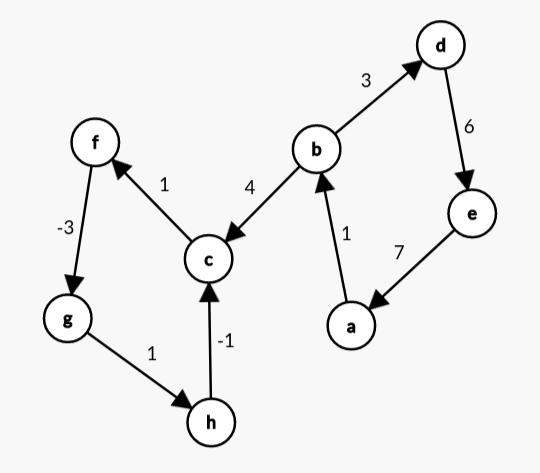
\includegraphics[width=0.8\linewidth]{figs/task-10/graph-10.png}
  \end{minipage}
  \begin{minipage}{0.5\textwidth}
    \centering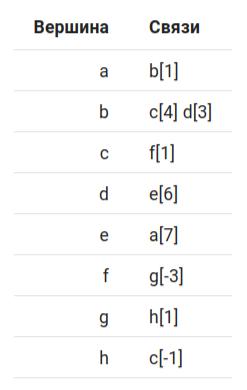
\includegraphics[width=0.5\linewidth]{figs/task-10/adj-10.png}
  \end{minipage}
  \caption{Ориентированный взвешенный граф}
\end{figure}

\begin{minted}{js}
{
  "weighted": true,
  "oriented": true,
  "adj": {
    "a": {
      "b": 1
    },
    "b": {
      "c": 4,
      "d": 3
    },
    "c": {
      "f": 1
    },
    "d": {
      "e": 6
    },
    "e": {
      "a": 7
    },
    "f": {
      "g": -3
    },
    "g": {
      "h": 1
    },
    "h": {
      "c": -1
    }
  }
}
\end{minted}

\subsubsection{Выходные данные}
\begin{figure}[H]
  \begin{minipage}{0.5\textwidth}
    \centering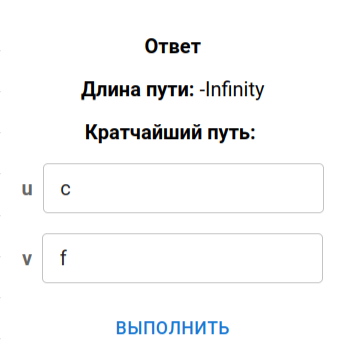
\includegraphics[width=0.7\linewidth]{figs/task-10/res-10-1.png}
  \end{minipage}
  \begin{minipage}{0.5\textwidth}
    \centering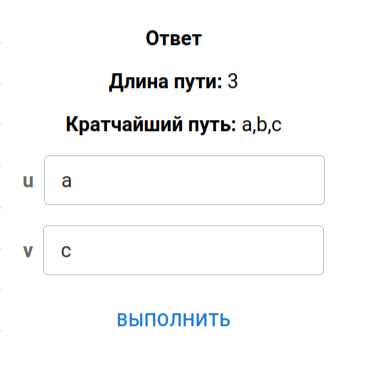
\includegraphics[width=0.7\linewidth]{figs/task-10/res-10-2.png}
  \end{minipage}
  \caption{Результат работы}
\end{figure}